\documentclass[12pt,a4paper]{article}
\usepackage{algorithm, algpseudocode, amsmath, amssymb, amsthm, bm, csquotes, emf, empheq, geometry, graphicx, hyperref, listings, mhchem, multirow, siunitx, slashbox, subcaption, upgreek}
\usepackage[italicdiff]{physics}
\usepackage[section]{placeins}
\usepackage[justification=centering]{caption}
\usepackage[column=O]{cellspace}
\usepackage[extrafootnotefeatures]{xepersian}
\hypersetup{colorlinks=true, urlcolor=cyan}

\title{تمرین سری سیزده دینامیک غیرخطی و آشوب}
\author{صالح شاملو احمدی}
\date{۱۲ خرداد ۱۴۰۲}

\settextfont{Yas}
\linespread{1.2}

\setlength\cellspacetoplimit{4pt}
\setlength\cellspacebottomlimit{3pt}
\newcommand{\multlinecell}[1]{\begin{tabular}[c]{@{}c@{}}#1\end{tabular}}

\newcommand{\qfrac}[2]{\left(\frac{#1}{#2}\right)}
\newcommand{\fsqrt}[2]{\sqrt{\frac{#1}{#2}}}
\newcommand{\ddfrac}[2]{{\displaystyle\frac{\displaystyle #1}{\displaystyle #2}}}
\newcommand{\pdvc}[3]{\qfrac{\partial #1}{\partial #2}_{#3}}
\newcommand{\dbar}{{d\mkern-7mu\mathchar'26\mkern-2mu}}
\newcommand*{\defeq}{\mathrel{\vcenter{\baselineskip0.5ex \lineskiplimit0pt
			\hbox{\scriptsize.}\hbox{\scriptsize.}}}
	=}

\newtheorem{theorem}{قضیه}
\newtheorem{lemma}{لم}
\renewcommand\qedsymbol{$\blacksquare$}

\begin{document}
	\maketitle
	\section{مسئله \lr{10.2.6}}
	\begin{figure}[h!]
		\centering
		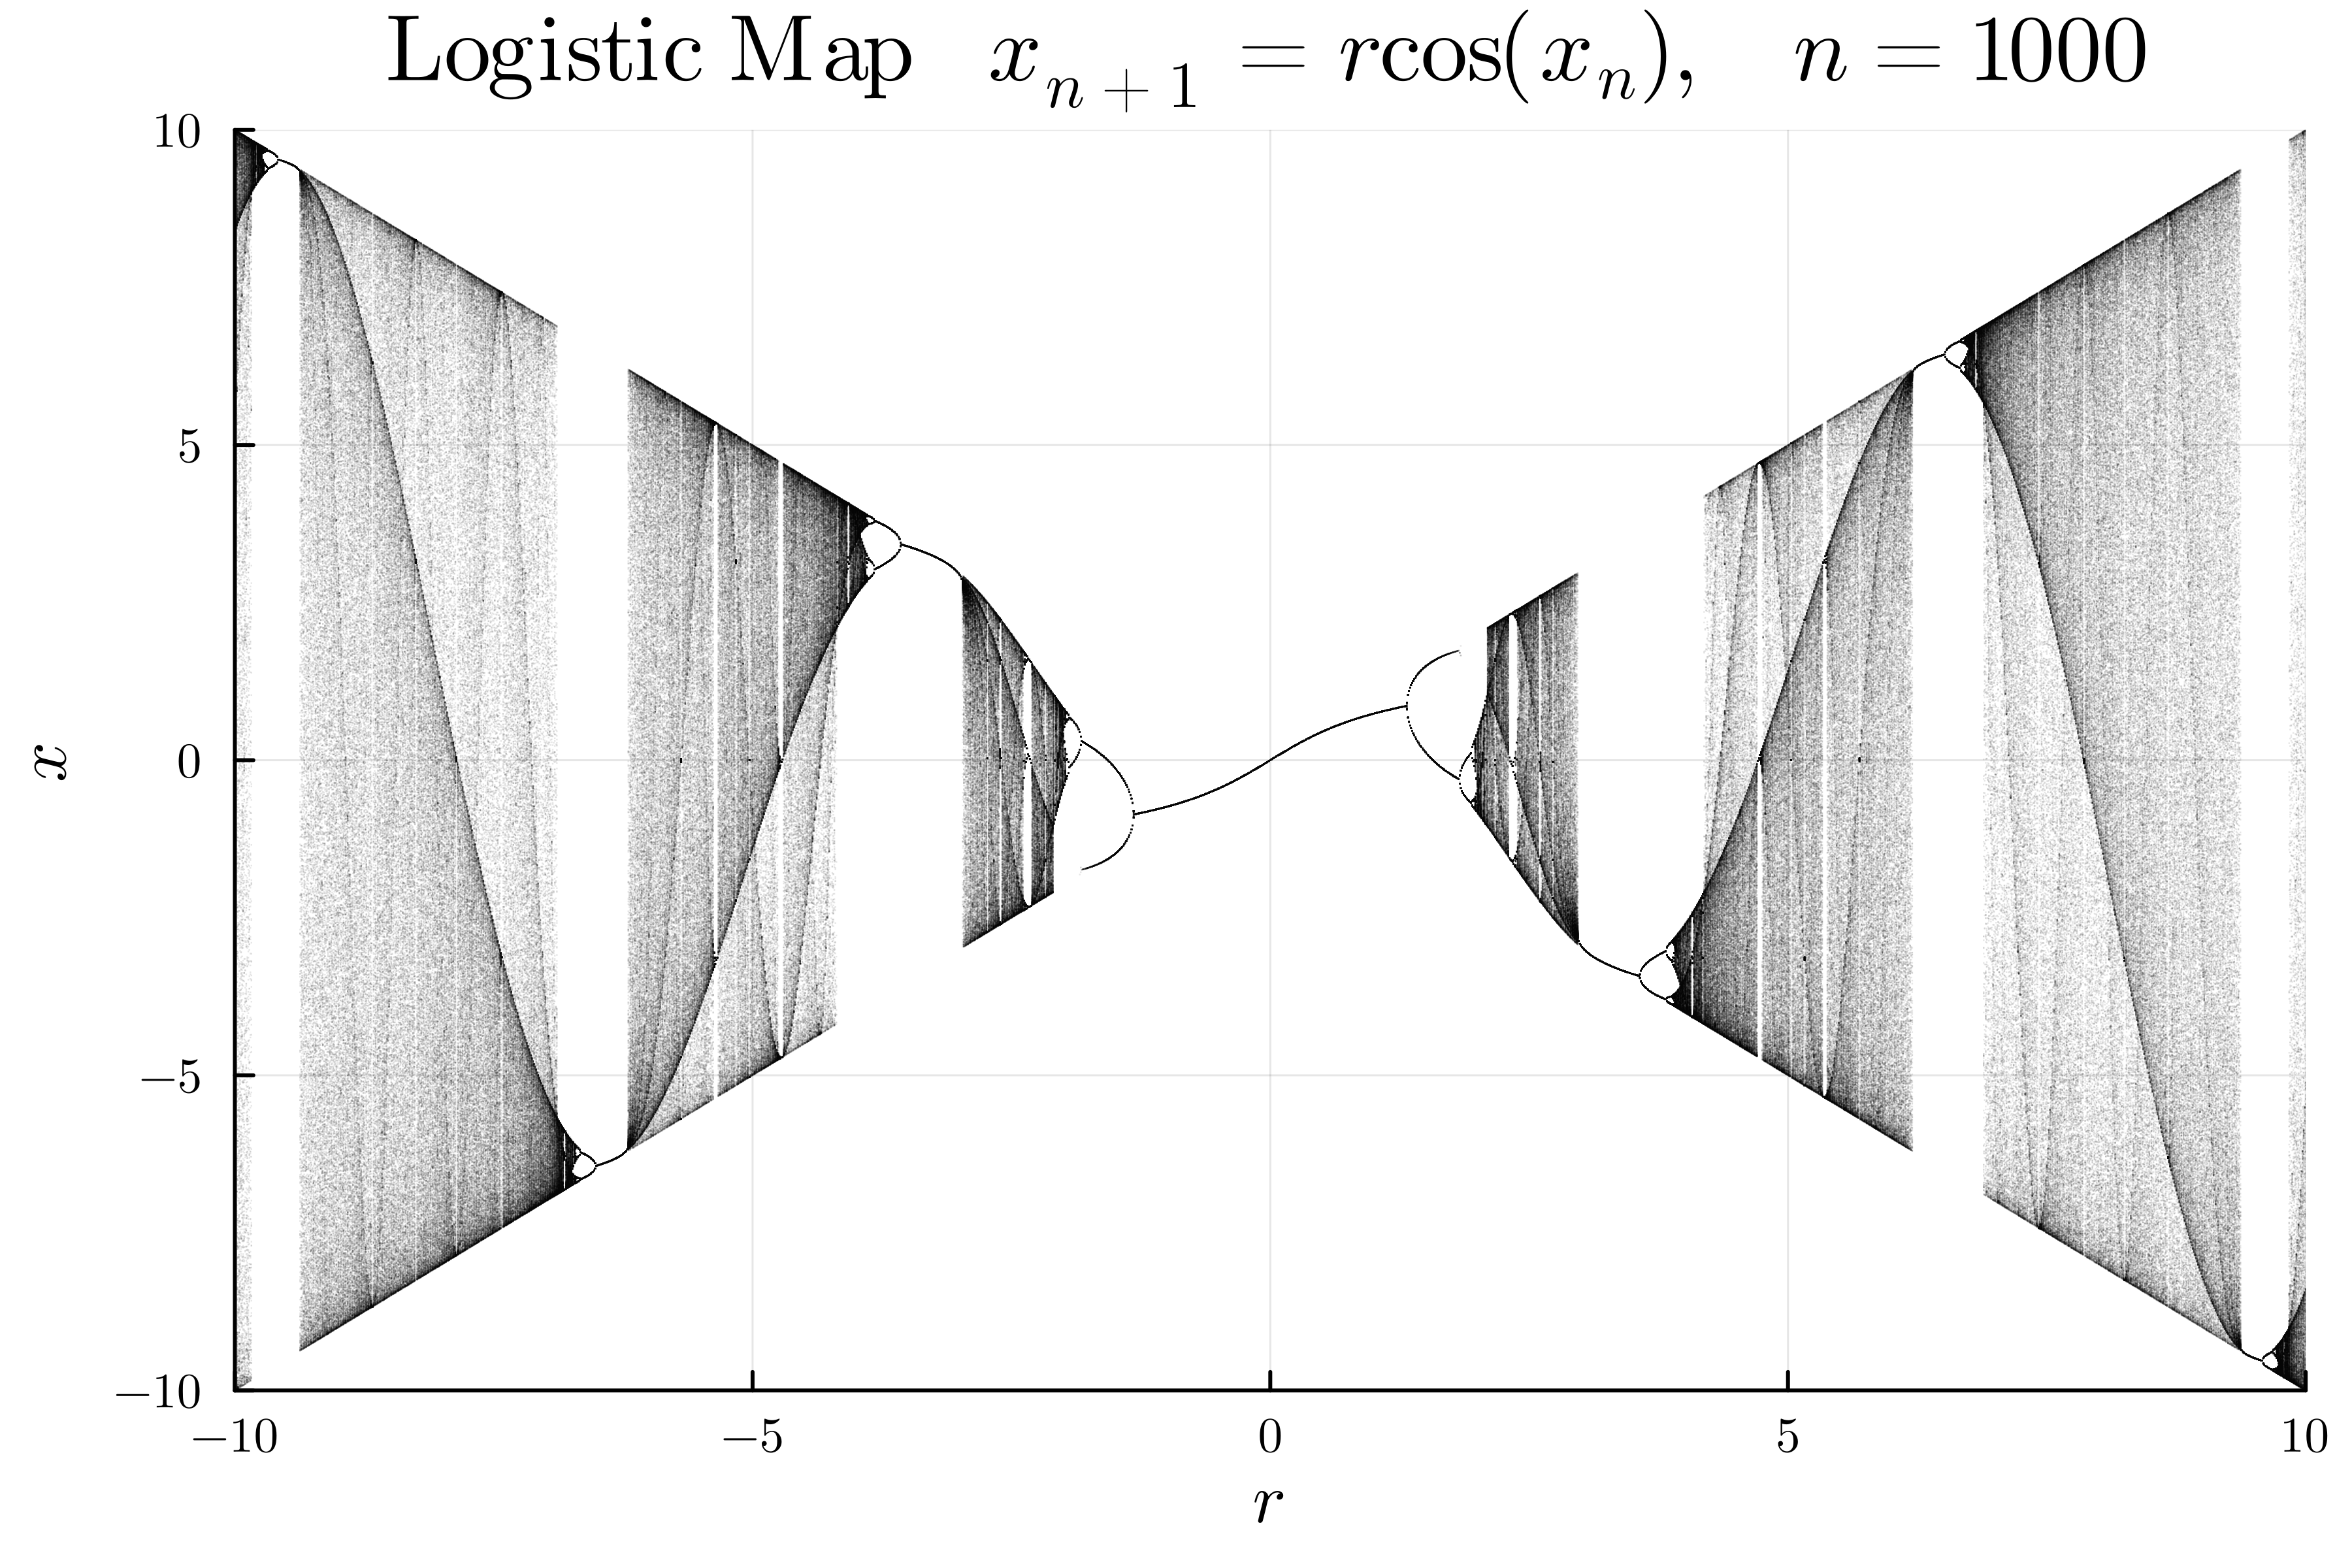
\includegraphics[width=\linewidth]{fig/10.2.6}
	\end{figure}
	
	\section{مسئله \lr{10.3.12}}
	\subsection{\lr{a}}
	\begin{equation}
		\dv{f}{x} = 0 \implies x = \frac{1}{2}
	\end{equation}
	بنابراین وقتی یک چرخه ابرپایدار است که نقطه $x=1/2 $ جزو آن باشد که معادل این است که $x=1/2 $ نقطه ثابتی برای
	تابع $f^{2^n}(x, r)$ باشد. بنابراین معادله ضمنی چرخه ابر پایدار بدین شکل است:
	\begin{equation}
		f^{2^n}(\frac{1}{2}, R_n) = \frac{1}{2}
	\end{equation}

	\subsection{\lr{b}}
	تا پنج رقم اعشار،
	\begin{align}
		R_2 &= 3.49856,\\
		R_3 &= 3.55464,\\
		R_4 &= 3.56667,\\
		R_5 &= 3.56924,\\
		R_6 &= 3.56980,\\
		R_7 &= 3.56991.
	\end{align}

	\subsection{\lr{c}}
	تا چهار رقم اعشار،
	\begin{equation}
		\delta \approx \frac{R_6 - R_5}{R_7 - R_6} = 4.6692.
	\end{equation}

	\section{مسئله \lr{10.4.9}}
	\begin{figure}[h!]
		\centering
		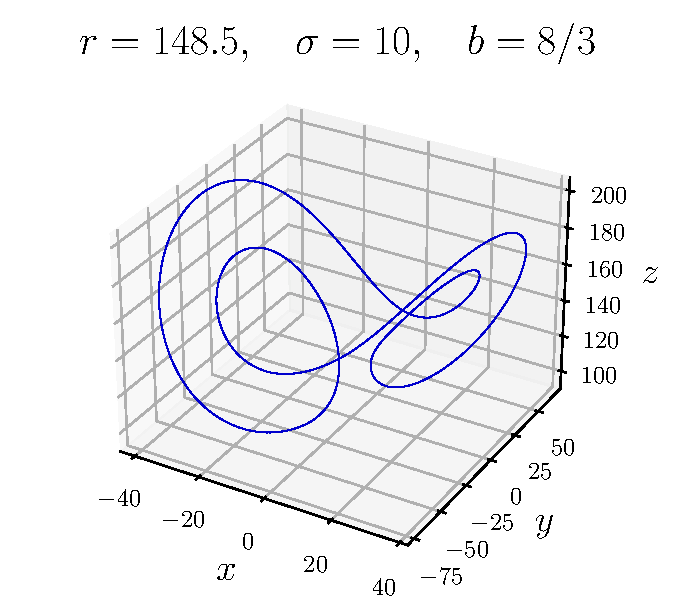
\includegraphics[width=0.7\linewidth]{fig/10.4.9.single.3d}
	\end{figure}
	\begin{figure}[h!]
		\centering
		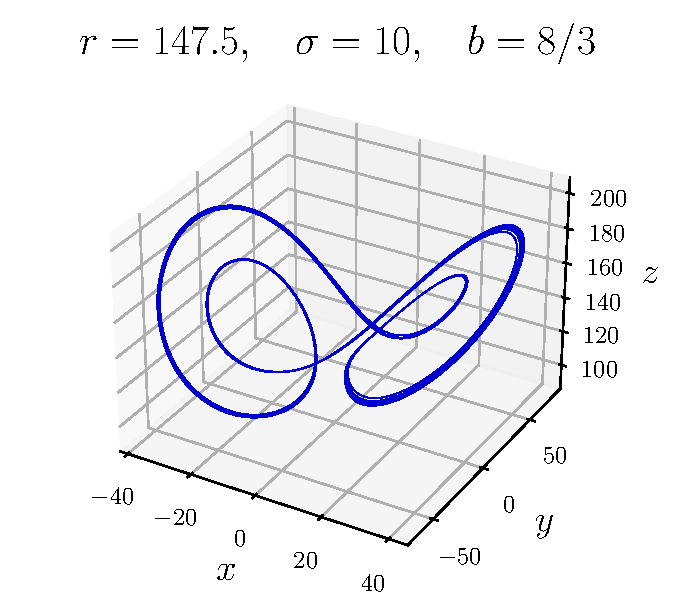
\includegraphics[width=0.7\linewidth]{fig/10.4.9.double.3d}
	\end{figure}
	\newgeometry{left=0.1in, right=0.1in, top=0.3in, bottom=0.3in}
	\begin{figure}[h!]
		\centering
		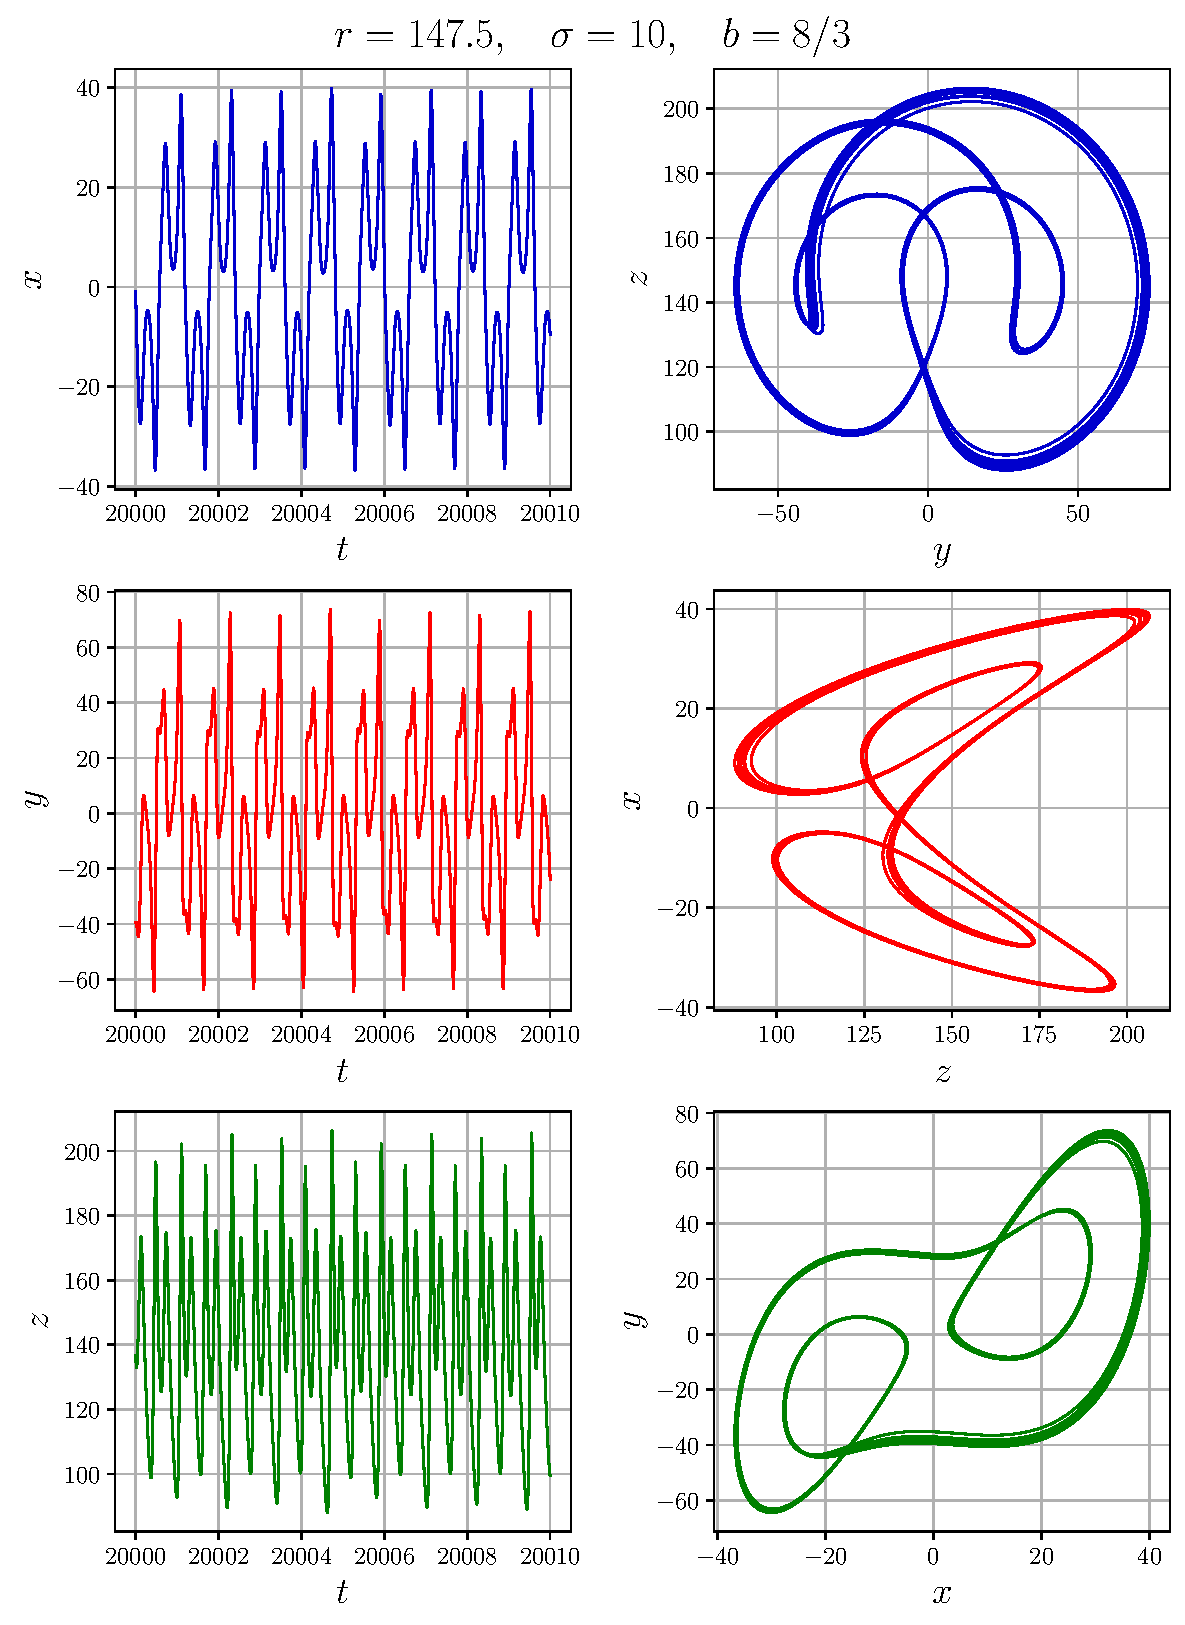
\includegraphics{fig/10.4.9.single}
	\end{figure}
	\begin{figure}[h!]
		\centering
		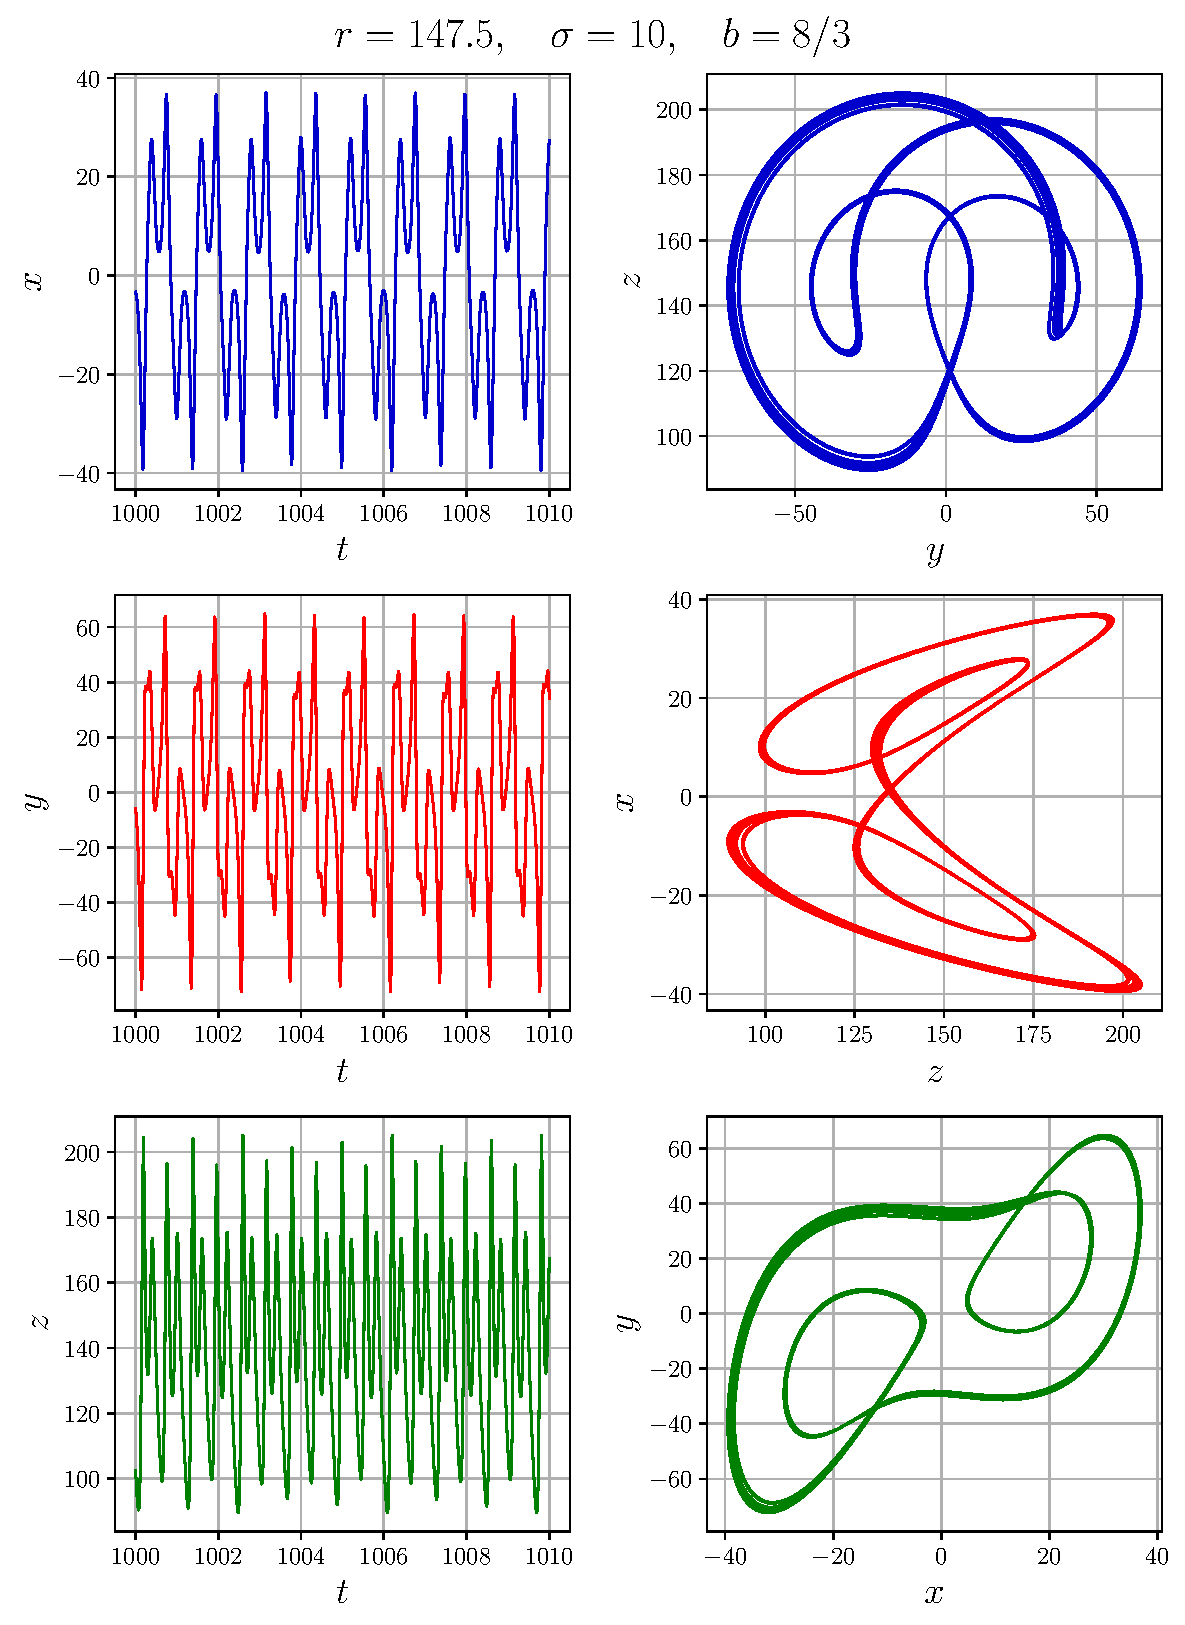
\includegraphics{fig/10.4.9.double}
	\end{figure}
	\restoregeometry
\end{document}